%%%%%%%%%%%%%%%%%%%%%%%%%%%%%%%%%%%%%%%%%%%%%%%%%%%
%
%  New template code for TAMU Theses and Dissertations starting Fall 2016.
%
%
%  Original Author: Sean Zachary Roberson
%  This version adapted for URS by Parasol lab.
%  Adapted from version 3.16.10, which was last updated on 9/29/2016.
%  URS adaptation last updated 1/9/2017.
%\part{title}
%%%%%%%%%%%%%%%%%%%%%%%%%%%%%%%%%%%%%%%%%%%%%%%%%%%

\documentclass[12pt]{report}

%These next lines change the font. Fixes for certain
%fonts will be implemented in a future release.

%Comment this line if you do not wish to use Times
%New Roman. The font used will then be the LaTeX
%default of Computer Modern.
\usepackage{times}
%\usepackage{cmbright}
\usepackage[T1]{fontenc}

%Do not change these settings. The geometry package
%Adjusts the margins to those specified by the Thesis
%Manual.
\usepackage[letterpaper]{geometry}
\geometry{verbose,tmargin=1.25in,bmargin=1.25in,lmargin=1.4in,rmargin=1.15in}
\usepackage[doublespacing]{setspace}
\usepackage{packages/tocloft}
\usepackage[rm, tiny, center, compact]{packages/titlesec}
\usepackage{indentfirst}
\usepackage{etoolbox}

\usepackage{packages/tocvsec2}
\usepackage[titletoc]{packages/appendix}
\usepackage{packages/appendix}
\usepackage{tamuconfig}

\usepackage{rotating}

%These are common AMS packages. Many LaTeX documents
%have these packages declared in their preambles.
\usepackage{amsmath, amsthm}

%This package allows for the use of graphics in the
%document.
\usepackage{graphicx}

%It is best practice to keep all your pictures in
%one folder inside the main directory in which your
%TeX file is kept. Here the folder is named "graphic."
%Replace the name here with your folder's name, if needed.
%The period is needed due to relative referencing.
\graphicspath{ {./graphic/} }

%If needed, this will allow you to add the word "Page"
%to extra pages on your front matter lists.
\usepackage{afterpage}

%This is from the mdwtools package; it fixes some
%footnote commands and allows you to have footnotes in
%tables via the savenotes environment.
\usepackage{footnote}
\usepackage{chngcntr}
\counterwithout{footnote}{chapter}


% Added to fix issues with pdf searching in some versions of LaTeX
%\usepackage[T1]{fontenc}\usepackage{lmodern}
%%%%%%%%%%%%%%%%%%%%%%%%%%%%%

% Hyperref setup below.  You should be able to get away with using uncommenting just the first line.
%\usepackage[hidelinks]{hyperref}

% if \usepackage[hidelinks]{hyperref} doesn't work try this.
%\usepackage{hyperref}  % Hidelinks is an option that removes link visiability.  TAMU Thesis Offices prefers to not see the links. But often doesn't work.
%
%\hypersetup{
%    colorlinks=true,
%    linkcolor=black,
%    citecolor=black,
%    filecolor=black,
%    urlcolor=black,
%}
%%%%%%%  End of hyperref setup.  One of these two options should work, but my motto with hyperref is when in doubt, comment it out!
%%%%%%%%%  This hopefully fixes the problem with vertical spacing of section headings at the top of the page..  Commented out in 1.0.7
% \preto\section{%
% \ifnum\value{section}>0\addtocontents{toc}{\vskip-6pt}\fi
% }
% \preto\subsection{%
% \ifnum\value{subsection}=0\addtocontents{toc}{\vskip-6pt}\fi
% \ifnum\value{subsection}>0\addtocontents{toc}{\vskip-6pt}\fi
% }
%%%%%%%%%%%%%%%%%%%%%%%%%%%%%%%%%%%%%%%%%%%%%%%%%%%%%%

\begin{document}

%The title of your document goes here.
%Spacing may need to be adjusted if your title is long
%and pushes the copyright off the page.
\renewcommand{\title}{Compatible Item Recommendation}

\newcommand{\abstracttitle}{Compatible Item Recommendation}

\renewcommand{\author}{Kevin J Nguyen \MakeLowercase{and} Victoria Wei}

%Your department name goes here.
\newcommand{\department}{Computer Science}

\newcommand{\program}{Undergraduate Research Scholar}

\newcommand{\ursadvisor}{James Caverlee}
\newcommand{\ursgradstudentadvisor}{Yin Zhang}
\newcommand{\advisordepartment}{Computer Science and Engineering}

% Doesn't change until next year.
\newcommand{\ursmonth}{May}
\newcommand{\ursyear}{2018}

%\titleformat{\chapter}[display]
%{\normalfont\bfseries\filcenter}{\chaptertitlename\
%\thechapter}{14pt}{\fontsize{14pt}{12pt}}

%%%%%%%%%%%%%%%%%%%%%%%%%%%%%%%%%%%%%%%%%%%%%%%%%%%
%
%  New template code for TAMU Theses and Dissertations starting Fall 2016.
%
%
%  Original Author: Sean Zachary Roberson
%  This version adapted for URS by Parasol lab.
%  Adapted from version 3.16.10, which was last updated on 9/29/2016.
%  URS adaptation last updated 1/9/2017.
%
%%%%%%%%%%%%%%%%%%%%%%%%%%%%%%%%%%%%%%%%%%%%%%%%%%%

%%%%%%%%%%%%%%%%%%%%%%%%%%%%%%
%% TITLE PAGE
%% The values get updated automatically.  Please do not make changes to this file other than adding/deleting committee members where necessary.
%%%%%%%%%%%%%%%%%%%%%%%%%%%%%%

\providecommand{\tabularnewline}{\\}



\begin{titlepage}

\begin{center}
\MakeUppercase{\textbf{\large{\title}}}
\vspace{4em}

An Undergraduate Research Scholars Thesis

by

\MakeUppercase{\author}

\vspace{4em}

\begin{singlespace}

Submitted to the Undergraduate Research Scholars program at\\
Texas A\&M University \\

in partial fulfillment of the requirements for the designation as an\\

\end{singlespace}

\vspace{2em}
\MakeUppercase{\program}
\par\end{center}

\begin{singlespace}
  \begin{tabular}{ll}
    & \tabularnewline & \cr
  \end{tabular}
\end{singlespace}

\begin{center}
  \vspace{\baselineskip}
  \begin{singlespace}
    Approved by Research Advisor:\hfill~Dr.~\ursadvisor
  \end{singlespace}
  \vspace{\baselineskip}
\end{center}

\begin{center}
\ursmonth \hspace{2pt} \ursyear

\vspace{3em}

Major: \department \par

\vspace{3em}

\par\end{center}
\end{titlepage}
\pagebreak{}




 % This is simply a file that formats and adds your titlepage, please do not edit this unless you have a specific need. .

%%%%%%%%%%%%%%%%%%%%%%%%%%%%%%%%%%%%%%%%%%%%%%%%%%%
%
%  New template code for TAMU Theses and Dissertations starting Fall 2016.
%
%
%  Original Author: Sean Zachary Roberson
%  This version adapted for URS by Parasol lab.
%  Adapted from version 3.16.10, which was last updated on 9/29/2016.
%  URS adaptation last updated 1/9/2017.
%
%%%%%%%%%%%%%%%%%%%%%%%%%%%%%%%%%%%%%%%%%%%%%%%%%%%
%%%%%%%%%%%%%%%%%%%%%%%%%%%%%%%%%%%%%%%%%%%%%%%%%%%%%%%%%%%%%%%%%%%%%%
%%       TABLE OF CONTENTS
%%%%%%%%%%%%%%%%%%%%%%%%%%%%%%%%%%%%%%%%%%%%%%%%%%%%%%%%%%%%%%%%%%%%%
% single-space sections in Table of Contents  - commented in version 1.7
%\renewcommand{\cftsecafterpnum}{\vskip0.5\baselineskip}
%\renewcommand{\cftsubsecafterpnum}{\vskip0.5\baselineskip}
%\renewcommand{\cftsubsubsecafterpnum}{\vskip0.5\baselineskip}
%%%%%%%%%%%%%%%%%%%%%%%%%%%%%%%%%%%%%%%%%%%%%%%%%%%

\phantomsection
\pagenumbering{gobble}
%\addcontentsline{toc}{chapter}{TABLE OF CONTENTS}

\begin{singlespace}
  \renewcommand\contentsname{\normalfont}
  {\centerline{{\textbf{\large{TABLE OF CONTENTS}}}}}

%\setcounter{tocdepth}{4} % This puts \subsubsection[]{×} in your List of Tables.  The default is 3.

\setcounter{tocdepth}{1}

%%%%%%%%%%%%%  Adds Page above the page number in TOC
\setlength{\cftaftertoctitleskip}{1em}
\renewcommand{\cftaftertoctitle}{%
\hfill{\normalfont {Page}\par}}


\tableofcontents

%\addtocontents{toc}{\protect\afterpage{~\hfill\normalfont{Page}\par\medskip}}
\end{singlespace}

\pagebreak{}
  % This adds the table of contents, please do not edit this unless you have a specific need.
%%%%%%%%%%%%%%%%%%%%%%%%%%%%%%%%%%%%%%%%%%%%%%%%%%%
%
%  New template code for TAMU Theses and Dissertations starting Fall 2016.
%
%
%  Original Author: Sean Zachary Roberson
%  This version adapted for URS by Parasol lab.
%  Adapted from version 3.16.10, which was last updated on 9/29/2016.
%  URS adaptation last updated 1/9/2017.
%
%%%%%%%%%%%%%%%%%%%%%%%%%%%%%%%%%%%%%%%%%%%%%%%%%%%
%%%%%%%%%%%%%%%%%%%%%%%%%%%%%%%%%%%%%%%%%%%%%%%%%%%%%%%%%%%%%%%%%%%%%
%%                           ABSTRACT
%%%%%%%%%%%%%%%%%%%%%%%%%%%%%%%%%%%%%%%%%%%%%%%%%%%%%%%%%%%%%%%%%%%%%

\chapter*{ABSTRACT}

\addcontentsline{toc}{chapter}{ABSTRACT} % Needs to be set to part, so the TOC doesnt add 'CHAPTER ' prefix in the TOC.

\pagestyle{plain} % No headers, just page numbers
\pagenumbering{arabic} % Arabic numerals
\setcounter{page}{1}
\begin{center}

\begin{singlespace}
\abstracttitle
\end{singlespace}
\vspace{2em}
\begin{singlespace}
\author \\
Department of \department \\
Texas A\&M University \\
\end{singlespace}
\vspace{2em}
\begin{singlespace}
Research Advisor: Dr. \ursadvisor \\
Department of \advisordepartment \\
Texas A\&M University \\
\end{singlespace}
\end{center}
\vspace{2em}

% \indent Recommending compatible items to users is an increasingly important research topic, and recommender systems are used extensively in different applications varying across domains to recommend items from books to music. e-Commerce systems such as Amazon and Netflix depend on recommender systems to increase their profits by recommending products the consumers are interested in against other products.

% \indent Current recommender systems recommend items based on two factors: user and items. For example, if a user buys a certain product, then the recommendation system will recommend similar products or products you have already purchased. For certain categories, the focus of compatibility relationship between products should be analyzed and used to recommend products to offer a complementary product, not just a similar product.

% \indent Our research proposes that compatibility can provide more accurate recommendations versus traditional recommender systems. This is especially true for electronics, so we will focus our research on electronics initially, and given time, we will progress to other categories. Through compatibility recommender systems, we will define compatibility for electronics, create a model to identify compatible products in electronics, analyze large product datasets and their relationships, and create a method to provide analytics for our results with recommender systems. Furthermore, our research differs from current market recommendation systems in that we will propose a recommendation system focused on compatibility and efficiency of the systems to provide user results.

% \indent Our overall challenge after we have created a new definition of compatibility is to analyze features that give us information about compatibility. This information includes text information, such as descriptions and product names, and image data. Another challenge is we must consider specific distinguishing features such as brand names. Next, we will find relationships between features that will give an appropriate compatible recommendation from our existing definition compared with existing recommendation that utilizes similar substitution methods. 


\indent Item recommendation is an increasingly important research topic that focuses on analyzing the relationships between products to recommend items to users based on their preferences or previous activity. These systems are used extensively in different applications varying across domains to recommend items ranging from books to music. Many companies, such as Amazon, Netflix, and Spotify, leverage recommender systems to drive further engagement and revenue by delivering value through a scalable way of personalizing content for their users.

\indent Current recommender systems recommend items based on two factors: users and items. For example, if a user purchases a product, then the recommender system will recommend similar products based on the users' previous purchases or similar social circles. In certain domains, such as clothing and electronics, the focus of compatibility relationships between products should be analyzed and used to recommend products to offer a complementary product, not a similar one.

\indent In our thesis, we propose a new definition of compatibility to provide a new and improved recommender system strictly for item compatibility. Compared to traditional recommender systems, compatibility recommender systems provide more accurate item recommendations for users. Our thesis currently focuses on analyzing the compatibility relationships within top-level categories in Amazon data but can be applied to any domain where compatibility is important. In order to do so, we define a general definition of compatibility, analyze a large product dataset and map product relationships, create a model to identify compatible items, and compare our results with other models. We will be analyzing the Cell Phone & Accessories category with our compatibility definition. Compared to other recommender systems, our compatibility recommender system is able to recommend compatible items at a higher accuracy and can therefore be used to provide users with a more personalized experience.

\pagebreak{}

%%%%%%%%%%%%%%%%%%%%%%%%%%%%%%%%%%%%%%%%%%%%%%%%%%%
%
%  New template code for TAMU Theses and Dissertations starting Fall 2016.
%
%
%  Original Author: Sean Zachary Roberson
%  This version adapted for URS by Parasol lab.
%  Adapted from version 3.16.10, which was last updated on 9/29/2016.
%  URS adaptation last updated 1/9/2017.
%
%%%%%%%%%%%%%%%%%%%%%%%%%%%%%%%%%%%%%%%%%%%%%%%%%%%
%%%%%%%%%%%%%%%%%%%%%%%%%%%%%%%%%%%%%%%%%%%%%%%%%%%%%%%%%%%%%%%%%%%%%%
%%                           DEDICATION
%%%%%%%%%%%%%%%%%%%%%%%%%%%%%%%%%%%%%%%%%%%%%%%%%%%%%%%%%%%%%%%%%%%%%
\chapter*{DEDICATION}
\addcontentsline{toc}{chapter}{DEDICATION}  % Needs to be set to part, so the TOC doesnt add 'CHAPTER ' prefix in the TOC.


\begin{center}
\vspace*{\fill}
This thesis is dedicated to all of the hard-working individuals in the field of Web and Distributed Information Management in Computer Science, our families, and our friends.
\vspace*{\fill}
\end{center}

\pagebreak{}

%%%%%%%%%%%%%%%%%%%%%%%%%%%%%%%%%%%%%%%%%%%%%%%%%%%
%
%  New template code for TAMU Theses and Dissertations starting Fall 2016.
%
%
%  Original Author: Sean Zachary Roberson
%  This version adapted for URS by Parasol lab.
%  Adapted from version 3.16.10, which was last updated on 9/29/2016.
%  URS adaptation last updated 1/9/2017.
%
%%%%%%%%%%%%%%%%%%%%%%%%%%%%%%%%%%%%%%%%%%%%%%%%%%%


%%%%%%%%%%%%%%%%%%%%%%%%%%%%%%%%%%%%%%%%%%%%%%%%%%%%%%%%%%%%%%%%%%%%%%
%%                           ACKNOWLEDGEMENTS
%%%%%%%%%%%%%%%%%%%%%%%%%%%%%%%%%%%%%%%%%%%%%%%%%%%%%%%%%%%%%%%%%%%%%
\chapter*{ACKNOWLEDGEMENTS}
\addcontentsline{toc}{chapter}{ACKNOWLEDGEMENTS}  % Needs to be set to part, so the TOC doesnt add 'CHAPTER ' prefix in the TOC.


\indent We would like to thank and express sincere gratitude to Yin Zhang, our graduate student advisor, and Dr. James Caverlee, our advisor, for their countless efforts and contributions to our research. Their guidance helped us tremendously on our research, and we appreciate their extreme optimism and perseverance with us throughout the year.

\pagebreak{}

%%%%%%%%%%%%%%%%%%%%%%%%%%%%%%%%%%%%%%%%%%%%%%%%%%%
%
%  New template code for TAMU Theses and Dissertations starting Fall 2016.
%
%
%  Original Author: Sean Zachary Roberson
%  This version adapted for URS by Parasol lab.
%  Adapted from version 3.16.10, which was last updated on 9/29/2016.
%  URS adaptation last updated 1/9/2017.
%
%%%%%%%%%%%%%%%%%%%%%%%%%%%%%%%%%%%%%%%%%%%%%%%%%%%
%%%%%%%%%%%%%%%%%%%%%%%%%%%%%%%%%%%%%%%%%%%%%%%%%%%%%%%%%%%%%%%%%%%%%%
%%             CONTRIBUTORS AND FUNDING SOURCES
%%%%%%%%%%%%%%%%%%%%%%%%%%%%%%%%%%%%%%%%%%%%%%%%%%%%%%%%%%%%%%%%%%%%%
\chapter*{CONTRIBUTORS}
\addcontentsline{toc}{chapter}{CONTRIBUTORS}  % Needs to be set to part, so the TOC doesn't add 'CHAPTER ' prefix in the TOC.


%This section is taken directly from the MS Word templates.

%Old version below.

%All theses and dissertations must include a contributors and funding sources section. In this section, name all members of the dissertation committee, and any collaboration with others in carrying out your thesis or dissertation research. Your independent contributions must be made clear.
%
%If financial support from the university or any other source was gained to conduct your thesis or dissertation research and compilation, it must be listed in this section. If you completed all work independently without outside financial support, indicate this here.
%\textit{(Sample Wording)}
%
%This work was supported by a dissertation committee consisting of Professor XXX [advisor – also note if co-advisor] and XXXX of the Department of [Home Department] and Professor(s) XXXX of the Department of [Outside Department].
% 
%The data analyzed for Chapter III was provided by Professor XXXX. The analyses depicted in Chapter IV were conducted in part by Rebecca Jones of the Department of Biostatistics and were published in (year) in an article listed in the Biographical Sketch. 
%
%All other work conducted for the dissertation was completed by the student independently.
%
%\noindent \textit{(or)}
%
%This work was supervised by a dissertation committee consisting of Professor XXXX [advisor – also note if co-advisor] and Professor(s) XXXX of the Department of [Home Department] and Professor(s) XXXX of [Outside Department]. All work for the dissertation was completed independently by the student.
%
%\noindent \textit{(or)}
%
%Graduate study was supported by a fellowship from Texas A\&M University and a dissertation research fellowship from XXX Foundation.

\subsection*{Contributors}
This work was supported by a thesis committee consisting of advisor Professor James Caverlee and graduate student Yin Zhang of the Department of Computer Science.

The data analyzed for our thesis was provided by Professor Julian McAuley from the Department of Computer Science at the University of California San Diego. 

All other work conducted for the thesis was completed by the students independently.
\pagebreak{}

%%%%%%%%%%%%%%%%%%%%%%%%%%%%%%%%%%%%%%%%%%%%%%%%%%%
%
%  New template code for TAMU Theses and Dissertations starting Fall 2016.
%
%
%  Original Author: Sean Zachary Roberson
%  This version adapted for URS by Parasol lab.
%  Adapted from version 3.16.10, which was last updated on 9/29/2016.
%  URS adaptation last updated 1/9/2017.
%
%%%%%%%%%%%%%%%%%%%%%%%%%%%%%%%%%%%%%%%%%%%%%%%%%%%
%%%%%%%%%%%%%%%%%%%%%%%%%%%%%%%%%%%%%%%%%%%%%%%%%%%%%%%%%%%%%%%%%%%%%%
%%                           SECTION I
%%%%%%%%%%%%%%%%%%%%%%%%%%%%%%%%%%%%%%%%%%%%%%%%%%%%%%%%%%%%%%%%%%%%%


\pagestyle{plain} % No headers, just page numbers
%\pagenumbering{arabic} % Arabic numerals
%\setcounter{page}{1}

\chapter{INTRODUCTION}

\indent The number of options people have access to is exponentially growing: millions of songs are available on Spotify, thousands of shows and movies are streamable online, and hundreds of restaurants are nearby. Due to the massive scale of the Internet, modern society provides people with a plethora of options to choose from. In the past, people shopped at physical stores, which are limited by the size of the store. By contrast, the Internet enables access to seemingly endless resources online. Amazon, for example, has an enormous collection of products but cannot display every product to every user. Due to the increase in information availability, the problem of displaying specific information to certain users arose. This gave way to information filtering systems and, more specifically, recommender systems.

For many companies, such as Amazon, Netflix, and Spotify, recommender systems drive further engagement and revenue by delivering value through a scalable way of personalizing content for their users. Modern recommender systems follow different paradigms for recommendation such as collaborative filtering, content-based recommendations, social/demographic recommendations, and contextual recommendations. Collaborative filtering compares the preferences of different users to generate predictions for users with similar preferences. Content-based recommendation leverages user preferences and domain-specific item content to generate new recommendations. Social and demographic recommendation utilizes preferences of friends, friends of friends, and demographics of similar people to suggest items. Furthermore, contextual recommendation provides recommendations based on the user's current context. For example, if a user is searching for a new car, car advertisements would be displayed and recommended as contextual recommendations.

% These paradigms typically focus on helping users discover similar items. Instead, we are interested in uncovering compatible items. For example, if a user purchases an iPhone 4, current recommender systems will recommend other similar iPhones. However, is there a way to recommend compatible iPhone 4 cases, chargers, or headphones? Although these items are not directly similar to an iPhone 4, these items should be considered equally as important to the end user since they are additional accessories that may be needed for the device and its functions.

These paradigms typically focus on helping users discover similar items. Modern recommender systems identify and understand the relationships between the items they recommend. In order to build a recommender system, a key component is that the system must have a clear definition on the relationships of items that are similar, substitutes, or complementary to develop a system that can understand a user`s intentions and recommend items \cite{linden-smith-york}.

To identify the relationships between items, this would require defining an appropriate distance or similarity measure between items or learning from training data to develop a model. Providing some metric to measure between similar items is suitable for determining an equivalence relation between items. This is to ensure that we recommend items that are considered substitutes to that item. However, a distance or similarity measure will propose issues where the compatibility between items is being considered. For example, two phone cases are similar in that they provide protection for a device and composition material, but they can be entirely different due to the devices they protect.

\section{Current Recommender Systems}
Currently, other research and industry has been aimed toward analyzing the compatibility relationships between products based on their visual appearance, textual descriptions, and ratings \cite{mcauley-pandey-leskovec, mcauley-targett-shi-hengel, menon-elkan}. Other research has used large data sets for training and provides complex models, but they follow the standard paradigm for machine learning and metric generation:

\begin{itemize}
    \item Collect a large dataset of related and unrelated items.
    \item Create a similarity function to provide distance or similarity constant.
    \item Train the function to determine related items are more similar than non-related.
\end{itemize}

These models provide a significant amount of information for distinguishing items that are similar and can range from topics of electronics to people \cite{dersaul}. The metric learning model is very flexible and powerful. However, it can ignore the details where compatibility should be considered. The current models themselves are not perfect and subject to limitations:

\begin{itemize}
    \item Similarity is either defined through an explicit category tree (e.g. `find the case nearest to this phone') and this subjects the model to noise and deficiencies in defined relations. Our model and algorithms would aim to solve this by performing recommendations without dependence on explicit relationship information.
    \item Model approaches are too strict in recommending different items. For example, an item cannot be compatible with itself or do not generate a diverse set of recommendations, such as recommending a similar product from a different brand. By analyzing the compatibility and relationships between products in a new and creative way, we can handle these issues.
\end{itemize}

Figure 1.1 describes an example of what `compatible' items would be recommended to the user given a set of queried products with a type of metric learning model: logistic regression. Logistic regression can be defined as follows.

\subsection{Logistic Regression}
Suppose $\mathbf{f}_i$ is the features that we get from product $i$ (which can be the concatenation of product image features, description features, and ratings). If $p$ is the probability that the two products are compatible, then

$$
logit(p) = b_0 + \beta \times \mathbf{X}_{ij}
$$

where $\mathbf{X}_{ij} = |\mathbf{f}_i - \mathbf{f}_j|$. 

\begin{figure}[h!]
\centering
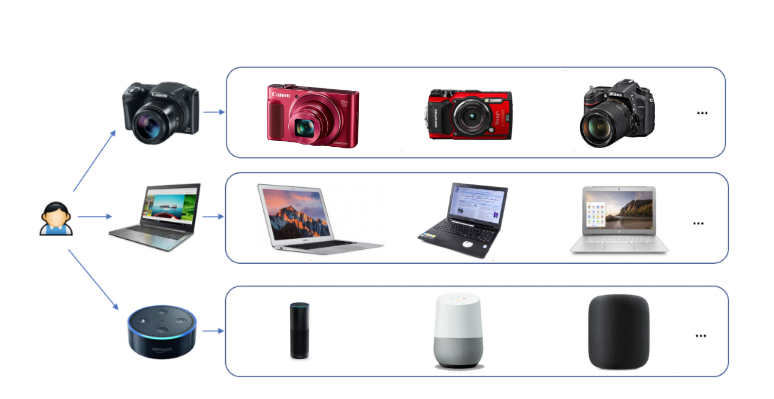
\includegraphics[scale=0.5]{data/LogisticRegression.png}
\caption{Diagram of the logistic regression model recommendations.}
\end{figure}

\section{Compatibility Recommender System}
In contrast, we are focused on discovering complementary items. For example, if a user purchases an iPhone 4, current recommender systems will recommend other similar iPhones. However, in many cases, recommending complementary items such as cases, chargers, or headphones is more relevant. Although these items are not directly similar to an iPhone 4, these items should be considered equally as important to the end user since they are additional accessories that may be needed for the device and its functions. Figure 1.2 shows an example of the compatible recommendations recommended from our compatibility classification model given the same set of queried products. 

\begin{figure}[h!]
\centering
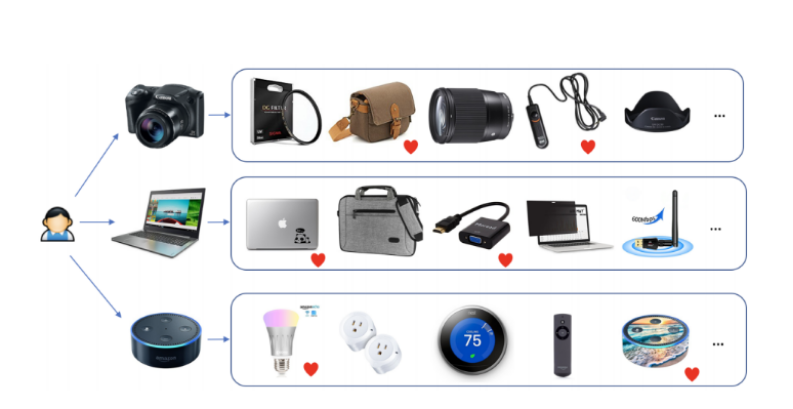
\includegraphics[scale=0.5]{data/CompatibilityModel.png}
\caption{Diagram of the compatibility model recommendations.}
\end{figure}

% For two items to be compatible, such as a phone and a charger or a dress and shoes, they must be similar in some ways but systematically different in others. Because compatibility is a human notion that is difficult to capture through the analysis of similar item relationships, compatibility of products is usually defined manually through expert individuals or assumed through the co-purchasing habits of customers. For example, if a customer buys an iPhone and then buys an iPhone charger, it is assumed that this iPhone and this iPhone charger are compatible. However, how about if this same customer purchases an iPhone and then a t-shirt? Are these now considered compatible? Therefore, it is not clear how to identify compatible items, especially for large and varied products sets. In a sample of 500,000 products in Electronics on Amazon, only 20\% explicitly mention “compatibility” with another product.2 Another challenging aspect is finding the number of items that are actually compatible with the queried product amongst a huge dataset. This could be less than 1\%! Thus, our research focuses on defining a new definition of compatibility in item recommender systems to provide scalable, improved item recommendation. 

For two items to be compatible, such as a phone and a charger or a dress and shoes, they must be similar in some ways but systematically different in others. Because compatibility is a human notion that is difficult to capture through the analysis of similar item relationships, compatibility of products is usually defined manually through expert individuals or assumed through the co-purchasing habits of customers, like on Amazon. In a sample of 500,000 products in Electronics on Amazon, only 20\% explicitly mention "compatibility" with another product, and therefore, assuming compatibility through co-purchasing habits can be very effective on a large scale but can be very prone to noise. For example, if a customer purchases an iPhone and an iPhone charger together, it is assumed that the iPhone and iPhone charger are compatible. However, the issue arises when a customer purchases two entirely unrelated products such as an iPhone and a t-shirt. The recommender system will now assume these two items are compatible when in reality they are not. Therefore, it is not clear how to correctly identify compatible items, especially for large and varied product sets. Another challenging aspect is finding the number of items that are compatible with the queried product among a huge dataset. Due to the large product data, randomly selecting an item has a less than 1\% chance of being compatible with the desired item. Thus, our research focuses on defining a new definition of compatibility in item recommender systems to provide scalable, improved item recommendation.

% In a sample of 500,000 products in Electronics on Amazon only 20\% explicitly mention "compatibility" with another product. Another challenging aspect is finding the number of items that are actually compatible with the queried product among a huge dataset. This could be less than 1\%! Thus, our research focuses on defining a new definition of compatibility in item recommender systems to provide scalable, improved item recommendation.

While using our improved item recommendation model, not only do customers have a more personalized space to do their shopping, but sellers also have a higher chance of being recommended to users, which may increase their revenue and product views. This is phenomenon is otherwise known as the cold-start problem. The cold-start problem is the issue where new products that are placed on the marketplace do not get as much attention as the older, more reviewed products. This is because of the co-purchasing effect, where items on Amazon are recommended based on customers and their buying techniques. Because these items are new and have not been bought with other items, the chances of these items making it into recommendation systems are very slim. However, our recommender system will solve this issue by not deriving compatibility from co-purchasing items but rather from the analysis of the product and its relation to other products in more concrete ways.

% In our research, we will propose new models and algorithms to identify the relationships between items in product recommendation settings. The new models and algorithms will utilize our definition of compatibility to create a more relevant and accurate way to recommend items.


%%%%%%%%%%%%%%%%%%%%%%%%%%%%%%%%%%%%%%%%%%%%%%%%%%%
%
%  New template code for TAMU Theses and Dissertations starting Fall 2016.
%
%
%  Original Author: Sean Zachary Roberson
%  This version adapted for URS by Parasol lab.
%  Adapted from version 3.16.10, which was last updated on 9/29/2016.
%  URS adaptation last updated 1/9/2017.
%
%%%%%%%%%%%%%%%%%%%%%%%%%%%%%%%%%%%%%%%%%%%%%%%%%%%
%%%%%%%%%%%%%%%%%%%%%%%%%%%%%%%%%%%%%%%%%%%%%%%%%%%%%%%%%%%%%%%%%%%%%%%
%%%                           SECTION II
%%%%%%%%%%%%%%%%%%%%%%%%%%%%%%%%%%%%%%%%%%%%%%%%%%%%%%%%%%%%%%%%%%%%%%



% \chapter{RELATED WORK}
% We relate our work in the context of prior studies and implementations of (1) item-to-item recommendations, e.g. systems that generate item-to-item recommendations by analyzing the relationship between items; and (2) studies involving metric learning including those not for recommendation.

% \section{Item-to-Item Recommendation}
% The analysis of the relationship among items is fundamental to modern real-world recommender systems, e.g. to generate recommendations of new songs on \textit{Spotify}. Most recommender systems utilize methods based on collaborative filtering, e.g. counting the overlap between users who have liked both songs, as in \textit{Spotify's} own solution \cite{madathil}. Other approaches include the use of latent-factor approaches that aim to model user-item relationships with low-dimensional factors to find recommendations with close embeddings. The systems that are able to predict the item-to-item relationship based on \textit{content} are most important to our research as the systems are proposed to address specific topics.

% Our work correlates with the co-purchase and co-browsing relationships using a dataset provided by \textit{Amazon} \cite{linden-smith-york}. We utilize previous works on these systems to provide quantitative results and compare our work against them. The main contribution of our work is to relax the model assumptions of current co-purchase and co-browsing systems to allow more complex relationships between items.

% \section{Metric Learning}
% The analysis of the relationship between objects is a vast topic that covers more topics than recommender systems. In modern learning, one is given a collection of relationships between items, and the goal is to identity a function that matches these relationships. The function must be able to generalize the relationship between objects and apply them to new unseen items to predict new relationships. The function is measured against valid data, and the metrics show how accurate the model can identify the relationships. The most developed and advanced learning methods are used to identify hidden variables or factors among items, through matrix-factorization or collaborative filtering. Again, our main goal is to relax the model assumption of current models and allow for more complex notions of `relatedness'. There are algorithms that work with non-metric learning of relationships, but to the extent of our knowledge do not scale well with larger sets of data.


\chapter{RELATED WORK} 

We relate our work in the context of prior studies and implementations of (1) item-to-item recommendations, e.g. systems that generate item-to-item recommendations by analyzing the relationship between items; (2) studies involving metric learning to build relationships between different sets of items; and (3) matrix factorization.

\section{Item-to-Item Recommendation}

The analysis of the relationship among items is fundamental to modern real-world recommender systems, e.g. to generate recommendations of new songs on \textit{Spotify}. As such, the closest systems to the compatibility recommender system we are proposing above are content-based recommender systems \cite{lew-sebe-djeraba-jain,adomavicius-tuzhilin} which attempt to model the user's preference toward items utilizing a variety of different features while using a similarity function, such as Pearson similarity \cite{melville}, cosine-based similarity \cite{deshpande}, and conditional probability-based similarity \cite{karypis}. These systems typically analyze the metadata from the user's previous activities and content. In comparison, other recommender systems utilize collaborative recommendation approaches, e.g. counting the overlap between users who have liked both songs, as in \textit{Spotify's} own solution \cite{madathil}. This type of recommendation allows the system to recommend items based off of similar user preferences and ratings, but requires a plethora of data in order to function effectively. In addition, item recommendation systems that utilize both content-based and collaborative techniques haven't been used to address the sparsity of data available and the cold-start problem (where products are invisible to the recommender system due to newness of the item) \cite{adomavicius-tuzhilin}. Other approaches for item-to-item recommendation incorporate additional features, such as images for fashion recommendation and phrase-level sentiment analysis.

The methods above determine the similarity between objects. In contrast, more research has been focused on detecting relationships between items that substitute or complement one another \cite{li-liu-huag}. For example, \cite{yin} focuses on the analysis of also-bought products and bought-together products to create compatibility relationships. \textit{Murillo et al.} analyzed photos of groups of people in social media to identify which groups of people are more likely to socialize, thus providing similarity distance measure between images \cite{urban-tribes}. \cite{ricci} provides more details on many of these types of recommender systems and challenges faced in this domain. Finally, \cite{adomavicius-tuzhilin} provides next-generation approaches on how to improve item recommendation. Our model provides a solution to many of these next-generation approaches. 

Unlike content-based recommender systems or collaborative filtering, our recommender system analyzes the content of items individually in a dataset and maps each item with a compatibility relationship to another item through entities defined by our definition of compatibility. Therefore, our recommender system does not need the preferences of other users and does not require the domain knowledge that content-based recommendations are derived from.

\section{Metric Learning}
The analysis of the relationship between objects is a vast topic that covers more domains than just recommender systems. In modern learning, one is given a collection of relationships between items, and the goal is to identify a function that matches these relationships. The function must be able to generalize the relationship between objects and apply them to new unseen items to predict new relationships. The function is measured against valid data, and the metrics show how accurate the model can identify the relationships created. The most developed and advanced learning methods are used to identify hidden variables or factors among items. This can be done through matrix-factorization or collaborative filtering. 

Utilizing metric learning, our main goal is to relax the model assumptions that current models have and allow for more complex notions of `relatedness'. There are algorithms that work with non-metric learning of relationships, but to the extent of our knowledge do not scale well with larger sets of data.

\section{Matrix Factorization}
Matrix Factorization is a concept used in recommendation systems that recommends items to users based on previous users and their rating patterns for specific items \cite{koren,koren-2}. Based on these rating patterns, higher positive ratings for items corresponding to users and their existing rating patterns will show a user's interest in that item and similar items. This will allow recommendation systems to detect what users will rate future items and whether or not such items should be recommended to the user \cite{koren,koren-2}. 

Matrix Factorization is just one of the methods for recommending items. However, in the world of compatibility, matrix factorization solely is unable to solve many of the challenges that compatibility presents. Matrix factorization shows user interest based on previous sentimental ratings, but this doesn't necessarily mean the items that the user rates positively are in any way compatible with each other. Our thesis aims to not only improve user interest but also increase existing compatibility nature between items.


%%%%%%%%%%%%%%%%%%%%%%%%%%%%%%%%%%%%%%%%%%%%%%%%%%%
%
%  New template code for TAMU Theses and Dissertations starting Fall 2016.
%
%
%  Original Author: Sean Zachary Roberson
%  This version adapted for URS by Parasol lab.
%  Adapted from version 3.16.10, which was last updated on 9/29/2016.
%  URS adaptation last updated 1/9/2017.
%
%%%%%%%%%%%%%%%%%%%%%%%%%%%%%%%%%%%%%%%%%%%%%%%%%%%
%%%%%%%%%%%%%%%%%%%%%%%%%%%%%%%%%%%%%%%%%%%%%%%%%%%%%%%%%%%%%%%%%%%%%%
%%                           SECTION III
%%%%%%%%%%%%%%%%%%%%%%%%%%%%%%%%%%%%%%%%%%%%%%%%%%%%%%%%%%%%%%%%%%%%%



\chapter{METHODS}

% In this chapter, we present the current problems with compatible item recommendation, and we provide a model aiming to solve these issues.

In this chapter, we present the problem of compatible item recommendation, and then, we present the design of our compatible item recommendation model.

\section{Problem Statement and Research Plan}
Given a set of items $I$ = $\{I_1, I_2, ... I_{|I|}\}$, we are trying to determine for each item $i$ in $I$ a set of compatible items $C_i$ = $\{ I_{c_1}, I_{c_2}, ... I_{|c_i|} \}$. Specifically, we are utilizing a large real-world dataset provided by Amazon introduced in \cite{mcauley-targett-shi-hengel} which features over a million products and 42 million co-purchased relationships across 20 top-level categories. We focus on the category of Cell Phone \& Accessories due to the prevalence of a variety of compatible characteristics. More specifically, we analyze all of the relationships between products in the top-level category of Cell Phone \& Accessories and their subcategories in order to find the compatible set $C_i$ for each product $i \in I$. We want to note here that although we are doing this analysis with just the Cell Phone \& Accessories category, this compatibility model can be applied to all top-level categories in the Amazon dataset. To accomplish our problem statement, we separate our solution into three parts: (i) define our definition of compatibility; (ii) classify each product with a specific product entity; (iii) utilize our compatibility classification to model complex compatible relationships.

\section{Defining Compatibility}

\begin{figure}[h!]
\begin{tabular}{ |p{6cm}|p{3cm}| }
 \hline
 \multicolumn{2}{|c|}{Sub-Category Compatibility} \\
 \hline
 Name & Type \\
 \hline
 Cases & Size \\
 Bluetooth Headsets & Interconnectivity \\
 Wired Headsets & Interconnectivity \\
 Chargers & Interconnectivity \\
 Cell Phone & Size \& Interconnectivity \\
 Screen Protectors & Size \\
 Internal Batteries & Size \& Interconnectivity \\
 External Battery Packs & Interconnectivity \\
 Battery Charger Cases & Size \& Interconnectivity \\
 Data Cables & Interconnectivity \\
 Smart Watches and Accessories & Interconnectivity \\
 \hline
\end{tabular}
\caption{Selected Cell Phone \& Accessories Sub-Categories and Type of Compatibility}
\end{figure}

In this section, we will define our definition of compatibility utilizing the type of relationships between top-level categories, their sub-categories, and the relationship within sub-categories. First, we organized each of the 20 top-level categories by their unique sub-categories and hand defined each sub-category's relation between each other and itself. For example, varying cases will be a size compatibility constraint, while varying chargers will be an interconnectivity compatibility constraint. Figure 3.1 describes this in more detail. There are some examples where size and interconnectivity both play a role in defining compatibility for a specific product. For example, the sub-category battery charger cases have both a size and interconnectivity component; the case has to be compatible with the size of the phone while the charger has to be compatible with the interconnectivity of the phone. While defining these relationships, we took caution to only consider the core functionality of the sub-categories, e.g. a case must be based on size and not fashion-sense. As a result, our definition of compatibility is derived from the relationship between sub-categories within top-level categories and comes in two forms: size and interconnectivity, for a specific product.

\subsection{Size}
As part of our definition of compatibility, we define size compatibility as the relationship between product $x$ and product $y$ such that $x$ and $y$ are strictly related to each other based on their physical appearance and dimensions while requiring that $x$ and $y$ both have the same top-level category. However, that means that $x$ and $y$ do not necessarily have to be in the same sub-category. In fact, it is crucial that $x$ and $y$ are in differing sub-categories for compatibility to be apparent. For example, an iPhone 4 and an iPhone 4 case belongs to the same Cell Phone \& Accessories top-level category. However, an iPhone 4 Case may belong to the sub-category of Cases, while an iPhone 4 may belong to the sub-category of Cell Phone. Therefore, the iPhone 4 and iPhone 4 Case have a size compatibility relationship. However, because an iPhone 4 and an iPhone 4s are both classified under the same sub-category of Cell Phone, they are not size compatible with one another.

\subsection{Interconnectivity}
Furthermore, we define interconnectivity compatibility as the relationship between product $x$ and product $y$ such that $x$ and $y$ are strictly related to each other based on their potential connectivity with each other while still requiring that $x$ and $y$ both have the same top-level category. However,there are many products in the same sub-category as $x$ that may not be interconnectivity compatible with $y$. For example, an iPhone 4 charging cable belongs to the sub-category of Data Cables in Cell Phone \& Accessories and has an interconnectivity compatibility relationship with the iPhone 4 in the Cell Phone sub-category in Cell Phone \& Accessories, but an iPhone 7 in the same Cell Phone sub-category in Cell Phone \& Accessories is not interconnectivity compatible with the same charging cable. To solve this, we develop a product entity classification that utilizes a natural language platform and our classification schema to build relationships between interconnectivity compatible products.

\section{Product Entity Classification}
\begin{figure}[h!]
    \begin{tabular}{ |p{0.5cm}|p{5cm}|p{4cm}|p{3cm}| }
     \hline
     \multicolumn{4}{|c|}{Sample Products} \\
     \hline
      & Name & Category & Entity \\
     \hline
     1 & Apple iPhone 4 AT\&T 16GB White & Cell Phone \& Accessories > Cell Phone  & Apple iPhone 4 \\
     2 & iPhone 4 Hello Kitty Case & Cell Phone \& Accessories > Cases & Apple iPhone 4 \\
     3 & Samsung S3 USB Cable & Cell Phone \& Accessories > Cables & Samsung Galaxy S3 \\
     \hline
    \end{tabular}
    \caption{Sample Products and their entity classification. The symbol '>' denotes a subcategory relationship.}
\end{figure}

After the classification of size and interconnectivity of sub-categories within top-level categories, we strengthen our definition of compatibility by classifying each product in each of these sub-categories with an entity. This entity will allow us to build our compatibility model and decide which products are compatible with other products. 

In Figure 3.2, we see sample products with their respective entity classifications. These classifications are necessary to decide size and interconnectivity compatible items. For example, product 1 belongs to the sub-category of Cell Phone while product 3 belongs to the sub-category of Cables. These items would be considered compatible if not for the interconnectivity compatibility definition. However, because these entities are different, we classify that product 1 and product 3 are not compatible. As another example, consider product 1 and product 2. Product 1 and product 2 belong in different sub-categories under the same top-level category Cell Phone \& Accessories. However, their entities are identical, classifying product 1 and product 2 to be compatible with each other. Our classification schema classifies over 340,000 products in this manner.


\subsection{Product Entity Classification}
In order to derive the product entity information, we utilized a natural language processing platform along with our classification model to recognize different entities of each product. After analyzing the benefits of multiple services, such as IBM Watson and Microsoft Cognitive Services, we decided to leverage the Google Cloud Natural Language Platform (GCL) due to the platform's ease of use, rapid response time, and consistent results. First, we analyzed the title and description of each product and queried GCL with this result. GCL then classifies each of the products into multiple entities based on product resemblance. Entities that GCL were able to classify include CONSUMER GOOD, ORGANIZATION, PERSON, LOCATION, EVENT, and etc. We used these entities, specifically CONSUMER GOOD, to decide what type of product the queried product was. In our case, CONSUMER GOOD was the only entity that described products that were purchasable objects. Using this entity, we found multiple amounts of CONSUMER GOOD entities for each product. To be more accurate in our classification, we decided to find the CONSUMER GOOD entity with the highest salience or accuracy percentage. In this way, we are able to be more accurate with our product entity classification model in analyzing what each product actually is and what items are compatible with each product. This CONSUMER GOOD entity corresponds to the entity that is in Figure 3.2.

We mapped each product to its highest CONSUMER GOOD salient entity. With this information, we created the product entity mapping for each product. 

\section{Compatibility Classification}
\begin{figure}[h!]
	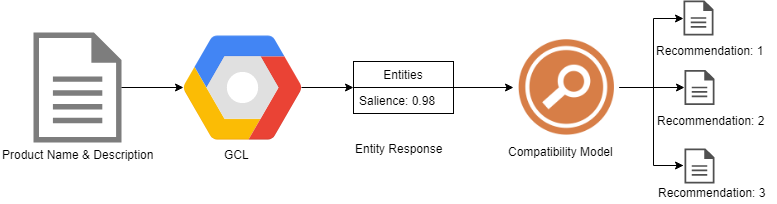
\includegraphics[scale=0.5]{data/Diagram.png}
	\caption{Item compatible recommendation work flow.}
\end{figure}

Utilizing the mapped product data in conjunction with the sub-category classification, we designed a compatibility classification model as follows. Each product has an entity mapping created by our classification model along with GCL. With this entity mapping, we are able to analyze compatible products, which are products that share the same entity but are in different sub-categories with the same top-level category. These are the items we would recommend the user. 

New products seeking compatibility recommendations are passed through GCL by title and description to get specific entities for that product. From there, the highest CONSUMER GOOD salient entity is gathered from the list of entities and is matched to our model to find other products that are compatible with the same CONSUMER GOOD salient entity. Next, we leverage all of the other sub-categories under the same top-level category of each item that is analyzed with the matching CONSUMER GOOD salient entity. From there, we return a subset of items from each sub-category as compatible items based on interconnectivity and size. Figure 3.3 shows a pictorial representation of our model and work flow. In this way, a variety of products cross-sub-category is recommended to the user that is compatible with the original product.


% For example, an iPhone 4 in the Cell Phone \& Accessories top-level category is not size compatible with a case for a Samsung Galaxy S3 even though the top-level category is size compatible with the sub-category of cases. Therefore, we must determine the entity in which each product is associated with. For example, the product 'Apple iPhone 4 AT&T 16GB White' belongs to Cell Phone \& Accessories and the product 'iPhone 4 Hello Kitty Case' belongs to the sub-category of Cases.


% For example, a product with title 'Apple iPhone 4 AT&T 16GB White' and 'iPhone 4 Hello Kitty Case' both belong to the entity of 'iPhone 4' are therefore are compatible. 


% Therefore, at the core of our research is the definition of compatibility. The difficulty arises from the novelty of the problem. Current recommender systems utilize collaborative filtering or content based recommendations as a metric for their recommendations. Compatibility is a human notion and therefore  


% \indent  Defining a new definition of compatibility is our biggest problem. This may be difficult because we have to research about what it means for something to be compatible by nature. Once we have figured out that definition, another challenge is to find ways of evaluating this new definition. This is a challenge because current evaluations of recommender systems use collaborative filtering efforts based on social-based recommendations. However, because ours is not of this form, we will have to devise new ways of implementing this. Finally, our last challenge is to define features that we will use to test this new definition of compatibility. We are proposing to test a range of electronics so that we can understand which electronics may be the most compatible with one another and if compatibility is really the best way of recommending electronics to users.

% \indent Another main challenge to note here is the cold start problem. The cold start problem is the problem that occurs when a new product is introduced. Because traditional recommender systems recommend compatible items based on co-purchasing, this new product has a very low chance of having any recommendations associated with it. This new product also has a very low chance of being recommended from other product selections. Our definition will solve the cold start problem by not relying on co-purchasing of items and instead focusing on text recognition and categories from the dataset to create a new definition of compatibility. Cold start problem doesn't affect how we determined annd defined our definition of compatibility.

% To accomplish this problem statement, we separate our solution into two parts. The first part is the text recognition platform, and the second part is the compatibility classification that we designed that contributes to our new definition of compatibility.

% \section{Method}

% \indent We first started by developing an idea about compatibility. In more depth, we wanted to see which products were compatible with other products. We searched through the Amazon dataset sorted by categories, and we created various documents based on the compatibility relationship between products in the same categories.  As a result, we developed a new notion - compatibility comes in two forms: size and interconnectivity.

% \subsection{Size}
% \indent As part of our definition of compatibility, we define size compatibility as products that fit together based on their physical appearance and dimensions. For example, an iPhone 4 is compatible with an iPhone 4 case but not an iPhone 7 case. Another example could be socks that are compatible with certain shoes based on shoe size.

% \subsection{Interconnectivity}
% \indent We define interconnectivity within our definition of compatibility as products that are compatible based on their connection with each other. For example, an iPhone 4 is compatible with an iPhone 4 charger, but an iPhone 7 is not compatible with this same iPhone 4 charger. Another example is a Macbook that is compatible with a traditional MagSafe Macbook charger but is not compatible with a Dell laptop charger.

% \indent To create this new definition of compatibility between items with these two classifications, we broke our solution down into two separate parts. The first part is the natural language platform that we used to recognize text and description of products, and the second part is the compatibility classification that we designed.

% \subsection{Natural Language Platform}
% \indent The text recognition platform that we have decided to use in conjunction with our compatibility model is the Google Cloud Natural Language Platform, otherwise known as GCL. We will use GCL to classify the text and description for each of the products in our dataset. This will allow our model to decide what kinds of products we are receiving from the dataset. Using this text recognition platform, we are to classify the overall key phrase for products in the same category. The natural language platform that we have decided to use in conjunction with our compatibility model is the Google Cloud Natural Language Platform. We will use the Google Cloud Natural Language Platform with our own model to classify the text and description for each of the products in our dataset. This will allow our model to decide what kinds of products we are receiving from the dataset. 

% \subsection{Compatibility Classification}
% \indent The compatibility classification model that we have designed is as follows. We take parts of the text-recognition classification. In particular, we are looking at the product with the highest salience in the consumer good entity. This is so that we can compare and contrast different consumer good entities to find out which of these products are compatible. If they share the same consumer good entity, then there is a higher probability that they are indeed compatible. However, an issue arises if they are the same or similar products. In this case, these products are not compatible. To solve this issue, we introduce the concept of categories. Using this natural language platform, we analyzed over 340,000 products and developed a classification schema that classifies each product in the dataset with key phrases that will contribute to the compatibility of that product based on the two notions of size and interconnectivity. We then develop relationship mappings between all products in the Amazon dataset based on our classifiers. After completion of this new definition of compatibility, if a user queries a product, our definition returns compatible recommendations for the user to choose and favorite. 


% \indent In our Amazon dataset, each product is labeled with categories and subcategories in which they belong in. For example, an iPhone case belongs in the category `Cell Phone & Accessories' and a subcategory `Cases'. Therefore, we can check compatibility by checking the categories of each of these products with the same consumer good classifier. If these categories are the same, then these products are classified as `similar' items and should not be compatible or recommended as compatible. If these categories are different, then this means that they are compatible in some shape or form. Therefore, we will recommend at least one product from each of the different categories in the same overall category. In this way, a variety of products cross-sub-category can be recommended to the user. 

% \indent We will introduce variables in both the natural language platform and the Amazon dataset. Figure 3.1 and 3.2 represent the variables for the corresponding models.

% The natural language platform has many variables, including... However, for the purposes of our research, we will only be looking at the salience value of the highest consumer good entity that we find in the platform classification as well as the name of the consumer good classifier. 

% The Amazon dataset also has many variables, including... However, for the purposes of our research, we will only be looking at the product name, description, categories, and also-bought items. 

% We will now discuss what these variables will be used for.



% %Fix table labeling.
% \begin{table}[h!]
% 	\centering
% 	\caption{San Japan attendance. Data is taken from \cite{ANCONS}. I intentionally make the title of this table long so the single space effect is seen in the list of tables.}
%         \vspace{1em}
% 	\begin{tabular}{|l|l|}
% 		\hline
% 		Dates & Attendance  \\ \hline
% 		August 8-10, 2008 & 3,523  \\ \hline
% 		August 14-16, 2009 & 4,003 \\ \hline
% 		July 9-11, 2010 & 5,049 \\ \hline
% 		August 5-7, 2011 & 6,891  \\ \hline
% 		August 10-12, 2012 & 9,464  \\ \hline
% 		August 16-18, 2013 & 11,077  \\ \hline
% 		July 18-20, 2014 & 14,686 \\ \hline
% 		July 31-August 2, 2015 & 18,411  \\ \hline
% 	\end{tabular}
% \end{table}

% You may be wondering why San Japan was chosen. There are a few reasons as to why I did this:

% \begin{enumerate}
% \item It is one of the fastest-growing anime conventions in Texas.
% \item Filler.
% \item I wanted a good variety of table examples.
% \item Because conventions are cool.
% \end{enumerate}

% The \textit{enumerate} environment was used to generated an ordered list above.

% \section{Section Test Example}
% We insert another figure here, just for kicks.

% \begin{figure}[h!]
% 	\centering
% 	\includegraphics[scale=0.5]{LowPass_Filter_Design.png}
% 	\caption{A low pass filter design.}
% \end{figure}


%%%%%%%%%%%%%%%%%%%%%%%%%%%%%%%%%%%%%%%%%%%%%%%%%%%
%
%  New template code for TAMU Theses and Dissertations starting Fall 2016.
%
%
%  Original Author: Sean Zachary Roberson
%  This version adapted for URS by Parasol lab.
%  Adapted from version 3.16.10, which was last updated on 9/29/2016.
%  URS adaptation last updated 1/9/2017.
%
%%%%%%%%%%%%%%%%%%%%%%%%%%%%%%%%%%%%%%%%%%%%%%%%%%%
%%%%%%%%%%%%%%%%%%%%%%%%%%%%%%%%%%%%%%%%%%%%%%%%%%%%%%%%%%%%%%%%%%%%%%
%%                           SECTION IV
%%%%%%%%%%%%%%%%%%%%%%%%%%%%%%%%%%%%%%%%%%%%%%%%%%%%%%%%%%%%%%%%%%%%%

\chapter{SUMMARY AND CONCLUSIONS \label{cha:Summary}}

\section{Results}
In order to qualitatively test our compatibility recommender system, we randomly selected 7 products from the dataset and analyzed the compatibility of the recommendations returned from four models: random selection, baseline, also-bought, and our compatibility model. For each model, we experimented with 5 recommendations for each product, and we determined if each product was compatible with the other products or not.


\subsection{Random Selection Model}
The random selection model divided the Cell Phone \& Accessories into a uniform distribution, allowing each product to have an equal chance of being recommended. Due to the large dataset and variety of products offered by Amazon, we expect very few to none randomly selected compatible items.

\subsection{Baseline Model}
The baseline model is a machine learned model created with logistic regression to recommend compatible items.

\subsection{Also Bought Model}
The Amazon dataset includes metadata about purchasing information such as `products also purchased with $x$'. We include this model in comparison to our compatibility model as this is the standard that Amazon uses to currently recommend compatible items to users.

\subsection{Compatibility Model}
The compatibility model utilizes our new definition of compatibility to recommend compatible items to users.

\subsection{Data}
Figure 4.1 shows the results from our experiments.
\begin{figure}[h!]
    \begin{tabular}{ |p{2cm}|p{2.5cm}|p{2.5cm}|p{2.5cm}|p{2.5cm}| }
     \hline
     \multicolumn{5}{|c|}{Compatible Item Recommendation Accuracy} \\
     \hline
     Product & Random & Baseline & Also-Bought & Compatibility \\
     \hline
     1 & 0\% & 0\% & 0\% & 80\% \\
     2 & 0\% & 0\% & 0\% & 0\% \\
     3 & 20\% & 60\% & 50\% & 100\% \\
     4 & 0\% & 0\% & 0\% & 0\% \\
     5 & 0\% & 0\% & 0\% & 0\% \\
     6 & 0\% & 0\% & 0\% & 0\% \\
     7 & 20\% & 0\% & 60\% & 100\% \\
     \hline
     Avg & 5.71\% & 8.57\% & 15.71\% & 40\% \\
     \hline
    \end{tabular}
    \caption{Compatible item recommendation accuracy with random, baseline, also-bought, and our compatibility models; tested for compatibility against 7 randomly selected products.}
\end{figure}

\section{Analysis}
Overall, our model had an overall higher average accuracy when recommending compatible items compared to the other models. More specifically, our model beats the baseline state-of-the-art model by 31.43\% and the also-bought model by 24.29\%.  Compared to the random model, the compatibility model does significantly better (34.29\%). These numbers are expected because out of all the products in the dataset, only roughly 1\% are compatible with the actual product. Therefore the probability of finding compatible items with that queried product is very low.

\section{Discussion and Conclusion}
In conclusion, we utilized our definition of compatibility to create a new recommender system that leverages the human notion of compatibility to recommend items to users while capturing the complex relationship of compatibility through a mixture of metadata, natural language, and entity mappings. While there are many other existing methods for compatible item recommendation that suffer from limitations such as sparsity in review data or the cold-start problem (a recommender system cannot draw any inferences for users or items due to lack of sufficient information), our implementation allows us to avoid and relax these constraints. 

\section{Challenges}
There are millions of items but only a small fraction actually mention compatibility. Our model further improves these notions of compatibility by defining the relation between products, whereas the small fraction that mention compatibility do so in a generic sense. As we have mentioned earlier, another difficulty is out of all products offered, at max only 1\% of the products are compatible items with the queried product. Finding this 1\% of compatible products is challenging in a dataset of millions.

Another main challenge to note here is relaxing the constraint of the cold start problem. The cold start problem is the problem that occurs when a new product is introduced. Because traditional recommender systems recommend compatible items based on co-purchasing, this new product has a very low chance of having any recommendations associated with it. This new product also has a very low chance of being recommended from other product selections. Our definition solves the cold start problem by not relying on co-purchasing of products. Therefore, the cold start problem doesn't affect how we determine or define our definition of compatibility.

Sparsity in review data is also a very common challenge faced by many other compatibility recommender systems. However, our model also relaxes this problem by not focusing our attention to users, actions, and behaviors based on the querying user but on the meaning of the product itself and not based on other users and their habits. 

\section{Further Study}
Currently, we have a compatibility classification model for over 340,000 products. In order to broaden the scope of our classifier, we will look further into analyzing the relationships of compatibility for other datasets and see if these relationships can be learned through machine learning and neural methods. We can also improve our classifier by researching more in depth about natural language and creating our own natural language platform for text recognition. Finally, we could also incorporate matrix factorization along with our compatibility model to even further improve user and compatibility interests. We believe that we can do better to improve our accuracy and continue to make our definition of compatibility stronger in the future. 

% %%%%%%%%%%%%%%%%%%%%%%%%%%%%%%%%%%%%%%%%%%%%%%%%%%%
%
%  New template code for TAMU Theses and Dissertations starting Fall 2016.
%
%
%  Original Author: Sean Zachary Roberson
%  This version adapted for URS by Parasol lab.
%  Adapted from version 3.16.10, which was last updated on 9/29/2016.
%  URS adaptation last updated 1/9/2017.
%
%%%%%%%%%%%%%%%%%%%%%%%%%%%%%%%%%%%%%%%%%%%%%%%%%%%

%%%%%%%%%%%%%%%%%%%%%%%%%%%%%%%%%%%%%%%%%%%%%%%%%%%%%%%%%%%%%%%%%%%%%%
%%                           NOMENCLATURE
%%%%%%%%%%%%%%%%%%%%%%%%%%%%%%%%%%%%%%%%%%%%%%%%%%%%%%%%%%%%%%%%%%%%%

\chapter*{NOMENCLATURE}
\addcontentsline{toc}{chapter}{NOMENCLATURE}  % Needs to be set to part, so the TOC doesnt add 'CHAPTER ' prefix in the TOC.

%A note about aligning: These entries will align
%themselves according to the ampersand (&).
%No extra spaces are needed, as seen in some of
%the entries below.
\vspace{-0.5in}
	\begin{table}[htbp]
	    \begin{tabular}{@{}p{0.33\textwidth} p{0.62\textwidth}@{}}
		B/CS		&	Bryan and College Station\\	[2ex] %[2ex] provides double space between each row
		TAMU			&	Texas A\&M University\\	[2ex]
		SDCC & San Diego Comic-Con\\ [2ex]
		EVIL & Every Villain is Lemons\\ [2ex]
		EPCC & Educator Preparation and Certification Center at Texas A\&M University - San Antonio\\ [2ex]
		FFT & Fast Fourier Transform\\ [2ex]
		ARIMA & Autoregressive Integrated Moving Average\\ [2ex]
		%XXXXXXXX		&	This is an optional page. Random word to test how long the sentence can be? This is just for test purpose. The current setting aims to align left/right margin same as all other pages.\\	[2ex]
	    \end{tabular}%
	\end{table}

\pagebreak{}


% %%%%%%%%%%%%%%%%%%%%%%%%%%%%%%%%%%%%%%%%%%%%%%%%%%%
%
%  New template code for TAMU Theses and Dissertations starting Fall 2016.
%
%
%  Original Author: Sean Zachary Roberson
%  This version adapted for URS by Parasol lab.
%  Adapted from version 3.16.10, which was last updated on 9/29/2016.
%  URS adaptation last updated 1/9/2017.
%
%%%%%%%%%%%%%%%%%%%%%%%%%%%%%%%%%%%%%%%%%%%%%%%%%%%
%%%%%%%%%%%%%%%%%%%%%%%%%%%%%%%%%%%%%%%%%%%%%%%%%%%%%%%%%%%%%%%%%%%%%%
%%                           LIST OF FIGURES
%%%%%%%%%%%%%%%%%%%%%%%%%%%%%%%%%%%%%%%%%%%%%%%%%%%%%%%%%%%%%%%%%%%%%

\phantomsection
\addcontentsline{toc}{chapter}{LIST OF FIGURES}

\renewcommand{\cftloftitlefont}{\center\bf\large\MakeUppercase}

\setlength{\cftbeforeloftitleskip}{-12pt} %% Positions the LOF title vertically to match the chapter titles
\renewcommand{\cftafterloftitleskip}{12pt}


\renewcommand{\cftafterloftitle}{%
\\[4em]\mbox{}\hspace{2pt}FIGURE\hfill{\normalfont Page}\vskip\baselineskip}

\begingroup


\begin{center}
\begin{singlespace}
%% These values make the lof table entries appear double spaced between.
\setlength{\cftbeforechapskip}{0.4cm}
\setlength{\cftbeforesecskip}{0.30cm}
\setlength{\cftbeforesubsecskip}{0.30cm}
\setlength{\cftbeforefigskip}{0.4cm}
\setlength{\cftbeforetabskip}{0.4cm}

\listoffigures

\end{singlespace}
\end{center}

\pagebreak{}
  % This adds the list of figures, this is optional. To remove, add a comment '%' at the beggining of the line.
% %%%%%%%%%%%%%%%%%%%%%%%%%%%%%%%%%%%%%%%%%%%%%%%%%%%
%
%  New template code for TAMU Theses and Dissertations starting Fall 2016.
%
%
%  Original Author: Sean Zachary Roberson
%  This version adapted for URS by Parasol lab.
%  Adapted from version 3.16.10, which was last updated on 9/29/2016.
%  URS adaptation last updated 1/9/2017.
%
%%%%%%%%%%%%%%%%%%%%%%%%%%%%%%%%%%%%%%%%%%%%%%%%%%%
%%%%%%%%%%%%%%%%%%%%%%%%%%%%%%%%%%%%%%%%%%%%%%%%%%%%%%%%%%%%%%%%%%%%%%
%%                           lIST OF TABLES
%%%%%%%%%%%%%%%%%%%%%%%%%%%%%%%%%%%%%%%%%%%%%%%%%%%%%%%%%%%%%%%%%%%%%%
%
\phantomsection
\addcontentsline{toc}{chapter}{LIST OF TABLES}

\renewcommand{\cftlottitlefont}{\center\bf\large\MakeUppercase}

\setlength{\cftbeforelottitleskip}{-12pt} %% Positions the LOT title vertically to match the chapter titles

%Note that the similar parameter in the LOF is 12pt; this
%is intentional to make the spacing between the headers
%and the first entry look consistent.
\renewcommand{\cftafterlottitleskip}{1pt}


\renewcommand{\cftafterlottitle}{%
\\[4em]\mbox{}\hspace{2pt}TABLE\hfill{\normalfont Page}\vskip\baselineskip}

\begin{center}
\begin{singlespace}

%% These values make the lot table entries appear double spaced between.
\setlength{\cftbeforechapskip}{0.4cm}
\setlength{\cftbeforesecskip}{0.30cm}
\setlength{\cftbeforesubsecskip}{0.30cm}
\setlength{\cftbeforefigskip}{0.4cm}
\setlength{\cftbeforetabskip}{0.4cm}

\listoftables

\end{singlespace}
\end{center}
\endgroup
\pagebreak{}  % Need this for the pagenumbering to be correct.
  % This adds the list of tables, this is optional. To remove, add a comment '%' at the beginning of the line.

% \include{data/chapter1}
% \include{data/chapter2}
% %%%%%%%%%%%%%%%%%%%%%%%%%%%%%%%%%%%%%%%%%%%%%%%%%%%
%
%  New template code for TAMU Theses and Dissertations starting Fall 2016.
%
%
%  Original Author: Sean Zachary Roberson
%  This version adapted for URS by Parasol lab.
%  Adapted from version 3.16.10, which was last updated on 9/29/2016.
%  URS adaptation last updated 1/9/2017.
%
%%%%%%%%%%%%%%%%%%%%%%%%%%%%%%%%%%%%%%%%%%%%%%%%%%%
%%%%%%%%%%%%%%%%%%%%%%%%%%%%%%%%%%%%%%%%%%%%%%%%%%%%%%%%%%%%%%%%%%%%%%
%%                           SECTION IV
%%%%%%%%%%%%%%%%%%%%%%%%%%%%%%%%%%%%%%%%%%%%%%%%%%%%%%%%%%%%%%%%%%%%%

\chapter{SUMMARY AND CONCLUSIONS \label{cha:Summary}}

\section{Results}
In order to qualitatively test our compatibility recommender system, we randomly selected 7 products from the dataset and analyzed the compatibility of the recommendations returned from four models: random selection, baseline, also-bought, and our compatibility model. For each model, we experimented with 5 recommendations for each product, and we determined if each product was compatible with the other products or not.


\subsection{Random Selection Model}
The random selection model divided the Cell Phone \& Accessories into a uniform distribution, allowing each product to have an equal chance of being recommended. Due to the large dataset and variety of products offered by Amazon, we expect very few to none randomly selected compatible items.

\subsection{Baseline Model}
The baseline model is a machine learned model created with logistic regression to recommend compatible items.

\subsection{Also Bought Model}
The Amazon dataset includes metadata about purchasing information such as `products also purchased with $x$'. We include this model in comparison to our compatibility model as this is the standard that Amazon uses to currently recommend compatible items to users.

\subsection{Compatibility Model}
The compatibility model utilizes our new definition of compatibility to recommend compatible items to users.

\subsection{Data}
Figure 4.1 shows the results from our experiments.
\begin{figure}[h!]
    \begin{tabular}{ |p{2cm}|p{2.5cm}|p{2.5cm}|p{2.5cm}|p{2.5cm}| }
     \hline
     \multicolumn{5}{|c|}{Compatible Item Recommendation Accuracy} \\
     \hline
     Product & Random & Baseline & Also-Bought & Compatibility \\
     \hline
     1 & 0\% & 0\% & 0\% & 80\% \\
     2 & 0\% & 0\% & 0\% & 0\% \\
     3 & 20\% & 60\% & 50\% & 100\% \\
     4 & 0\% & 0\% & 0\% & 0\% \\
     5 & 0\% & 0\% & 0\% & 0\% \\
     6 & 0\% & 0\% & 0\% & 0\% \\
     7 & 20\% & 0\% & 60\% & 100\% \\
     \hline
     Avg & 5.71\% & 8.57\% & 15.71\% & 40\% \\
     \hline
    \end{tabular}
    \caption{Compatible item recommendation accuracy with random, baseline, also-bought, and our compatibility models; tested for compatibility against 7 randomly selected products.}
\end{figure}

\section{Analysis}
Overall, our model had an overall higher average accuracy when recommending compatible items compared to the other models. More specifically, our model beats the baseline state-of-the-art model by 31.43\% and the also-bought model by 24.29\%.  Compared to the random model, the compatibility model does significantly better (34.29\%). These numbers are expected because out of all the products in the dataset, only roughly 1\% are compatible with the actual product. Therefore the probability of finding compatible items with that queried product is very low.

\section{Discussion and Conclusion}
In conclusion, we utilized our definition of compatibility to create a new recommender system that leverages the human notion of compatibility to recommend items to users while capturing the complex relationship of compatibility through a mixture of metadata, natural language, and entity mappings. While there are many other existing methods for compatible item recommendation that suffer from limitations such as sparsity in review data or the cold-start problem (a recommender system cannot draw any inferences for users or items due to lack of sufficient information), our implementation allows us to avoid and relax these constraints. 

\section{Challenges}
There are millions of items but only a small fraction actually mention compatibility. Our model further improves these notions of compatibility by defining the relation between products, whereas the small fraction that mention compatibility do so in a generic sense. As we have mentioned earlier, another difficulty is out of all products offered, at max only 1\% of the products are compatible items with the queried product. Finding this 1\% of compatible products is challenging in a dataset of millions.

Another main challenge to note here is relaxing the constraint of the cold start problem. The cold start problem is the problem that occurs when a new product is introduced. Because traditional recommender systems recommend compatible items based on co-purchasing, this new product has a very low chance of having any recommendations associated with it. This new product also has a very low chance of being recommended from other product selections. Our definition solves the cold start problem by not relying on co-purchasing of products. Therefore, the cold start problem doesn't affect how we determine or define our definition of compatibility.

Sparsity in review data is also a very common challenge faced by many other compatibility recommender systems. However, our model also relaxes this problem by not focusing our attention to users, actions, and behaviors based on the querying user but on the meaning of the product itself and not based on other users and their habits. 

\section{Further Study}
Currently, we have a compatibility classification model for over 340,000 products. In order to broaden the scope of our classifier, we will look further into analyzing the relationships of compatibility for other datasets and see if these relationships can be learned through machine learning and neural methods. We can also improve our classifier by researching more in depth about natural language and creating our own natural language platform for text recognition. Finally, we could also incorporate matrix factorization along with our compatibility model to even further improve user and compatibility interests. We believe that we can do better to improve our accuracy and continue to make our definition of compatibility stronger in the future. 


%The next line is the format for inserting new sections.
%Replace the name "newsection"  with the name of your
%new section file.
%\include{data/newsection}


%fix spacing in bibliography, if any...
%%%%%%%%%%%%%%%%%%%%%%%%%%%%%%%%%%%%%%%%%%%%%%%%%%%%%%%%%%%%%
%\let\oldbibitem\bibitem
%\renewcommand{\bibitem}{\setlength{\itemsep}{0pt}\oldbibitem}
%%%%%%%%%%%%%%%%%%%%%%%%%%%%%%%%%%%%%%%%%%%%%%%%%%%%%%%%%%%%%%%
%The bibliography style declared is the IEEE format. If
%you require a different style, see the document
%bibstyles.pdf included in this package. This file,
%hosted by the University of Vienna, shows several
%bibliography styles and examples of in-text citation
%and a references page.

\phantomsection
\addcontentsline{toc}{chapter}{REFERENCES}

\renewcommand{\bibname}{{\large\rm\bf REFERENCES}}
%This file is a .bib database that contains the sources.
\bibliography{data/myReference}
\bibliographystyle{ieeetr}

%This next line includes appendices. The file
%appendix.tex contains commands pointing to
%the appendix files; be sure to change these
%pointers if you end up changing the filenames.
%Leave this commented if you will not need
%appendix material.

% %%
%% This is file `appendix.sty',
%% generated with the docstrip utility.
%%
%% The original source files were:
%%
%% appendix.dtx  (with options: `usc')
%% 
%% -----------------------------------------------------------------
%%   Author: Peter Wilson, Herries Press
%%   Maintainer: Will Robertson (will dot robertson at latex-project dot org)
%%   Copyright 1998--2004 Peter R. Wilson
%% 
%%   This work may be distributed and/or modified under the
%%   conditions of the LaTeX Project Public License, either
%%   version 1.3c of this license or (at your option) any
%%   later version: <http://www.latex-project.org/lppl.txt>
%% 
%%   This work has the LPPL maintenance status "maintained".
%%   The Current Maintainer of this work is Will Robertson.
%% 
%%   This work consists of the files listed in the README file.
%% -----------------------------------------------------------------
%% 
\NeedsTeXFormat{LaTeX2e}
\ProvidesPackage{appendix}[2009/09/02 v1.2b extra appendix facilities]

\newif\if@chapter@pp\@chapter@ppfalse
\newif\if@knownclass@pp\@knownclass@ppfalse
\@ifundefined{chapter}{%
  \@ifundefined{section}{}{\@knownclass@pptrue}}{%
  \@chapter@pptrue\@knownclass@pptrue}
\providecommand{\phantomsection}{}
\newcounter{@pps}
  \renewcommand{\the@pps}{\alph{@pps}}
\newif\if@pphyper
  \@pphyperfalse
\AtBeginDocument{%
  \@ifpackageloaded{hyperref}{\@pphypertrue}{}}

\newif\if@dotoc@pp\@dotoc@ppfalse
\newif\if@dotitle@pp\@dotitle@ppfalse
\newif\if@dotitletoc@pp\@dotitletoc@ppfalse
\newif\if@dohead@pp\@dohead@ppfalse
\newif\if@dopage@pp\@dopage@ppfalse
\DeclareOption{toc}{\@dotoc@pptrue}
\DeclareOption{title}{\@dotitle@pptrue}
\DeclareOption{titletoc}{\@dotitletoc@pptrue}
\DeclareOption{header}{\@dohead@pptrue}
\DeclareOption{page}{\@dopage@pptrue}
\ProcessOptions\relax
\newcommand{\@ppendinput}{}
\if@knownclass@pp\else
  \PackageWarningNoLine{appendix}%
    {There is no \protect\chapter\space or \protect\section\space command.\MessageBreak
     The appendix package will not be used}
  \renewcommand{\@ppendinput}{\endinput}
\fi
\@ppendinput

\newcommand{\appendixtocon}{\@dotoc@pptrue}
\newcommand{\appendixtocoff}{\@dotoc@ppfalse}
\newcommand{\appendixpageon}{\@dopage@pptrue}
\newcommand{\appendixpageoff}{\@dopage@ppfalse}
\newcommand{\appendixtitleon}{\@dotitle@pptrue}
\newcommand{\appendixtitleoff}{\@dotitle@ppfalse}
\newcommand{\appendixtitletocon}{\@dotitletoc@pptrue}
\newcommand{\appendixtitletocoff}{\@dotitletoc@ppfalse}
\newcommand{\appendixheaderon}{\@dohead@pptrue}
\newcommand{\appendixheaderoff}{\@dohead@ppfalse}
\newcounter{@ppsavesec}
\newcounter{@ppsaveapp}
\setcounter{@ppsaveapp}{0}
\newcommand{\@ppsavesec}{%
  \if@chapter@pp \setcounter{@ppsavesec}{\value{chapter}} \else
                 \setcounter{@ppsavesec}{\value{section}} \fi}
\newcommand{\@pprestoresec}{%
  \if@chapter@pp \setcounter{chapter}{\value{@ppsavesec}} \else
                 \setcounter{section}{\value{@ppsavesec}} \fi}
\newcommand{\@ppsaveapp}{%
  \if@chapter@pp \setcounter{@ppsaveapp}{\value{chapter}} \else
                 \setcounter{@ppsaveapp}{\value{section}} \fi}
\newcommand{\restoreapp}{%
  \if@chapter@pp \setcounter{chapter}{\value{@ppsaveapp}} \else
                 \setcounter{section}{\value{@ppsaveapp}} \fi}
\providecommand{\appendixname}{Appendix}
\newcommand{\appendixtocname}{Appendices}
\newcommand{\appendixpagename}{Appendices}
\newcommand{\appendixpage}{%
  \if@chapter@pp \@chap@pppage \else \@sec@pppage \fi
}
\newcommand{\clear@ppage}{%
  \if@openright\cleardoublepage\else\clearpage\fi}

\newcommand{\@chap@pppage}{%
  \clear@ppage
  \thispagestyle{plain}%
  \if@twocolumn\onecolumn\@tempswatrue\else\@tempswafalse\fi
  \null\vfil
  \markboth{}{}%
  {\centering
   \interlinepenalty \@M
   \normalfont
   \Huge \bfseries \appendixpagename\par}%
  \if@dotoc@pp
    \addappheadtotoc
  \fi
  \vfil\newpage
  \if@twoside
    \if@openright
      \null
      \thispagestyle{empty}%
      \newpage
    \fi
  \fi
  \if@tempswa
    \twocolumn
  \fi
}

\newcommand{\@sec@pppage}{%
  \par
  \addvspace{4ex}%
  \@afterindentfalse
  {\parindent \z@ \raggedright
   \interlinepenalty \@M
   \normalfont
   \huge \bfseries \appendixpagename%
   \markboth{}{}\par}%
  \if@dotoc@pp
    \addappheadtotoc
  \fi
  \nobreak
  \vskip 3ex
  \@afterheading
}

\newif\if@pptocpage
  \@pptocpagetrue
\newcommand{\noappendicestocpagenum}{\@pptocpagefalse}
\newcommand{\appendicestocpagenum}{\@pptocpagetrue}
\newcommand{\addappheadtotoc}{%
  \phantomsection
  \if@chapter@pp
    \if@pptocpage
      \addcontentsline{toc}{chapter}{\appendixtocname}%
    \else
      \if@pphyper
        \addtocontents{toc}%
          {\protect\contentsline{chapter}{\appendixtocname}{}{\@currentHref}}%
      \else
        \addtocontents{toc}%
          {\protect\contentsline{chapter}{\appendixtocname}{}}%
      \fi
    \fi
  \else
    \if@pptocpage
      \addcontentsline{toc}{section}{\appendixtocname}%
    \else
      \if@pphyper
        \addtocontents{toc}%
          {\protect\contentsline{section}{\appendixtocname}{}{\@currentHref}}%
      \else
        \addtocontents{toc}%
          {\protect\contentsline{section}{\appendixtocname}{}}%
      \fi
    \fi
  \fi
}

\providecommand{\theH@pps}{\alph{@pps}}

\newcommand{\@resets@pp}{\par
  \@ppsavesec
  \stepcounter{@pps}
  \setcounter{section}{0}%
  \if@chapter@pp
    \setcounter{chapter}{0}%
    \renewcommand\@chapapp{\appendixname}%
    \renewcommand\thechapter{\@Alph\c@chapter}%
  \else
    \setcounter{subsection}{0}%
    \renewcommand\thesection{\@Alph\c@section}%
  \fi
  \if@pphyper
    \if@chapter@pp
      \renewcommand{\theHchapter}{\theH@pps.\Alph{chapter}}%
    \else
      \renewcommand{\theHsection}{\theH@pps.\Alph{section}}%
    \fi
    \def\Hy@chapapp{\appendixname}%
  \fi
  \restoreapp
}

\newenvironment{appendices}{%
  \@resets@pp
  \if@dotoc@pp
    \if@dopage@pp              % both page and toc
      \if@chapter@pp           % chapters
        \clear@ppage
      \fi
      \appendixpage
    \else                      % toc only
       \if@chapter@pp          % chapters
         \clear@ppage
       \fi
      \addappheadtotoc
    \fi
  \else
    \if@dopage@pp              % page only
      \appendixpage
    \fi
  \fi
  \if@chapter@pp
    \if@dotitletoc@pp \@redotocentry@pp{chapter} \fi
  \else
    \if@dotitletoc@pp \@redotocentry@pp{section} \fi
    \if@dohead@pp
      \def\sectionmark##1{%
        \if@twoside
          \markboth{\@formatsecmark@pp{##1}}{}
        \else
          \markright{\@formatsecmark@pp{##1}}{}
        \fi}
    \fi
    \if@dotitle@pp
      \def\sectionname{\appendixname}
      \def\@seccntformat##1{\@ifundefined{##1name}{}{\csname ##1name\endcsname\ }%
        \csname the##1\endcsname\quad}
    \fi
  \fi}{%
  \@ppsaveapp\@pprestoresec}

\newcommand{\setthesection}{\thechapter.\Alph{section}}
\newcommand{\setthesubsection}{\thesection.\Alph{subsection}}

\newcommand{\@resets@ppsub}{\par
  \stepcounter{@pps}
  \if@chapter@pp
    \setcounter{section}{0}
    \renewcommand{\thesection}{\setthesection}
  \else
    \setcounter{subsection}{0}
    \renewcommand{\thesubsection}{\setthesubsection}
  \fi
  \if@pphyper
    \if@chapter@pp
      \renewcommand{\theHsection}{\theH@pps.\setthesection}%
    \else
      \renewcommand{\theHsubsection}{\theH@pps.\setthesubsection}%
    \fi
    \def\Hy@chapapp{\appendixname}%
  \fi
}

\newenvironment{subappendices}{%
  \@resets@ppsub
  \if@chapter@pp
    \if@dotitletoc@pp \@redotocentry@pp{section} \fi
    \if@dotitle@pp
      \def\sectionname{\appendixname}
      \def\@seccntformat##1{\@ifundefined{##1name}{}{\csname ##1name\endcsname\ }%
        \csname the##1\endcsname\quad}
    \fi
  \else
    \if@dotitletoc@pp \@redotocentry@pp{subsection} \fi
    \if@dotitle@pp
      \def\subsectionname{\appendixname}
      \def\@seccntformat##1{\@ifundefined{##1name}{}{\csname ##1name\endcsname\ }%
        \csname the##1\endcsname\quad}
    \fi
  \fi}{}

\newcommand{\@formatsecmark@pp}[1]{%
  \MakeUppercase{\appendixname\space
    \ifnum \c@secnumdepth >\z@
      \thesection\quad
    \fi
    #1}}
\newcommand{\@redotocentry@pp}[1]{%
  \let\oldacl@pp=\addcontentsline
  \def\addcontentsline##1##2##3{%
    \def\@pptempa{##1}\def\@pptempb{toc}%
    \ifx\@pptempa\@pptempb
      \def\@pptempa{##2}\def\@pptempb{#1}%
      \ifx\@pptempa\@pptempb
\oldacl@pp{##1}{##2}{\appendixname\space ##3}%
      \else
        \oldacl@pp{##1}{##2}{##3}%
      \fi
    \else
      \oldacl@pp{##1}{##2}{##3}%
    \fi}
}
\endinput
%%
%% End of file `appendix.sty'.


\end{document}
